\pgfplotsset{compat=1.17}

\section{MPAS-Atmosphere Result}
\label{sec:conc}

\subsection{C and MPI Compiler selection}
For our first approach, we've tested out different C and MPI compiler combination. The result shows ICC 2021.10.0 with OpenMPI 4.1.5 is the best suite for MPAS, which outperformed other combination when running MPAS on the 32 nodes. 

\begin{figure}[ht]
  \centering
  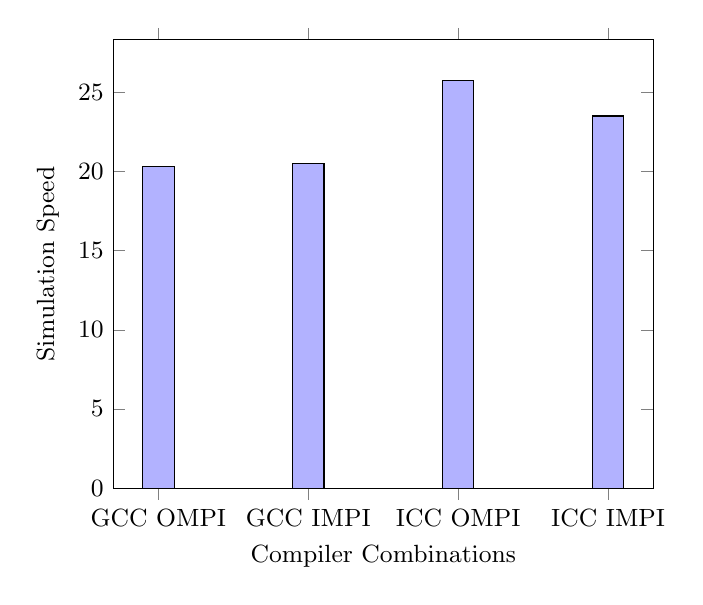
\begin{tikzpicture}
    \begin{axis}[
      ybar,
      bar width=0.4cm,
      xlabel={Compiler Combinations},
      ylabel={Simulation Speed},
      symbolic x coords={GCC OMPI, GCC IMPI, ICC OMPI, ICC IMPI},
      xtick=data,
      ymin=0,
      xticklabel style={font=\small},
      yticklabel style={font=\small},
      xlabel style={font=\small},
      ylabel style={font=\small},
    ]
      \addplot[fill=blue!30] coordinates {(GCC OMPI, 20.34) (GCC IMPI, 20.48) (ICC OMPI, 25.7474) (ICC IMPI, 23.5069)};
    \end{axis}
  \end{tikzpicture}
  \caption{ICC 2021.10.0 with OpenMPI 4.1.5 outperforms GCC with OpenMPI, GCC with IntelMPI and ICC 2021.10.0 with IntelMPI on the 32 nodes MPAS testcase.}
  \label{fig:bar_chart}
\end{figure}

\subsection{CPU Affinity}
With two CPUs on each node, we have to make sure the process binding is consisted during runtime, and the socket they are placing is correct. At the end, we chose to bind the core to hwthread and place them in the correct socket by --bind-to and --map-by from mpirun command line option. On the 32 nodes MPAS testcase, the average time is 0.3\% faster with process binding than without.

\subsection{Compile Time Flag}
We invoke the \texttt{-march}, \texttt{-ax}, and \texttt{-Ofast} flag in compiling. Since we know the architecture of the machine so setting the corresponding \texttt{-march} flag should have a significant performance increase. As the result, the first two flags really works well on MPAS, especially when \texttt{-march} flag is set to \texttt{core-avx2}. It shows the overall integration time is reduced by 4 seconds, which is almost a 10\% performance improvement. For the \texttt{-Ofast} flag, it didn't corrupt the result while it barely get any performance improvement.


\subsection{Link Time Flag}
As we are using Intel ICC compiler, we should always try the \texttt{-ipo} flag which enables multi-file interprocedural optimization in linking phase. Although we barely get any performance improvements after we tried, but theoretically, it should work well with a large application like MPAS.

\subsection{Parallel IO variables in MPAS}

In the running file of MPAS, a file called \texttt{namelist.atmosphere} stores the parameters used in simulation. There are two variables related to Parallel IO library is \texttt{config\_pio\_num\_tasks} and \texttt{config\_pio\_strides}. The fundamental rules to tune these two variables is to keep the product of them equals to the number of MPI tasks we used, which is

\begin{align*}
     config\_pio\_num\_tasks \times config\_pio\_strides\\
    = Total\;MPI\;tasks
\end{align*}

We tune these two parameters based on this equation, and tried with three different configurations, which are (32, 48), (48, 32), and (64, 24) for \texttt{config\_pio\_num\_tasks} and \texttt{config\_pio\_strides} respectively for 32 nodes (total 1536 MPI tasks). The result is shown in Fig.~\ref{fig:config-pio}.

\begin{figure}[htb]
    \centering
    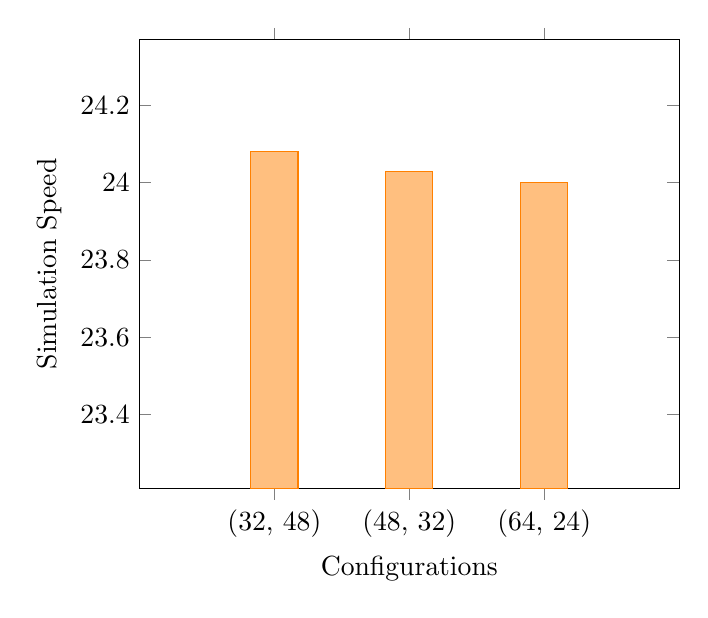
\begin{tikzpicture}
        \begin{axis}[
            ybar,
            bar width=0.6cm,
            xlabel={Configurations},
            ylabel={Simulation Speed},
            ymin=23.5,
            symbolic x coords={\text{(32, 48)}, \text{(48, 32)}, \text{(64, 24)}},
            xtick=data,
            enlargelimits=0.5,
        ]
        \addplot[
            color=orange,
            fill=orange,
            fill opacity=0.5
        ] coordinates {(\text{(32, 48)}, 24.08) (\text{(48, 32)}, 24.03) (\text{(64, 24)}, 24)};
        \end{axis}
    \end{tikzpicture}
    \caption{Simulation Speed with different PIO parameters in MPAS. All of them uses 32 nodes to get the best performance.}
    \label{fig:config-pio}
\end{figure}

We can see that when the configurations on these two parameters matches the nodes we used and the hardware threads on each machine, MPAS performances slightly better cause they matches the number of nodes and hardware threads performing I/O operations. We've gained about 0.3\% of performance increase from here.

\subsection{Graph Load-Balancing}
After all these basic compiler and related flag settings, we start to analyze the IPM profiling result. In Fig.~\ref{figure:profile-before} we found that the load-balancing didn't seem really well on MPAS. We guess it was caused by the way MPAS partitioning the mesh and it should be able to resolve by giving different Metis setup. 

\begin{figure}[h]
    \centering
    \includegraphics[width=0.5\textwidth]{profileBefore.JPG} 
    \caption{Load balancing of MPI functions according to simulation time (without I/O)}
    \label{figure:profile-before}
\end{figure}

After some research, we found that we were able to change the load balancing tolerance in Metis. Also, another important option is selecting \texttt{objtype} (the mesh optimize mode) from optimization for edge cuts to optimization for communication. After several tests, we discovered that the latter option always have a bit higher simulation speed.

\begin{table}[ht]
    \centering
    \caption{Metis Configuration Comparison}
    \begin{tabular}{lll}
        \toprule
        Type & Default & Optimize  \\
        \midrule
        Objtype & Edge Cuts (cut) & Communication (vol) \\
        Edge cuts & 350158 & 347823 \\
        Communication volume & 354760 & 352425 \\
        Balance & 1.015 & 1.004 \\
        \bottomrule
    \end{tabular}
    \label{table:metis-configuration}
\end{table}

Then, we profile again after our work. The balancing issue has improved a little bit since the peak in the graph has dropped from 1.6 to 1.4 in Fig.~\ref{figure:profile-after}. In conclusion, we got only 1\% faster in simulation time, but we believe it may impact more in some longer or larger testcases.

\begin{figure}[h]
    \centering
    \includegraphics[width=0.5\textwidth]{profile.JPG} 
    \caption{Load balancing of MPI functions according to simulation time (without I/O) after our approach}
    \label{figure:profile-after}
\end{figure}

\subsection{I/O optimization}
Due to the longer integration step occurring every simulated 10 minutes, we suspect that there may have I/O operations causing delays. Thus, we've tried different I/O optimization attempts to solve this issue. A simple attempt is set some ROMIO environment variables to boost up the I/O. By setting romio\_cb\_read or romio\_cb\_write, which can enable, disable or let the program select the activation of the collecting buffering. In our best approach, we enable both of them. This easy setup has saved a lot of time on waiting I/O events.

\subsection{OpenMPI and UCX Configuration}
One of the best way to have better performance is to have better communication tools. UCX and MPI configuration may be the most important part in CPU task. In UCX, we turn off all the debugging flags and also turn off the verbs support since it have worse performance than other methods in OpenMPI 4.1.5. Moreover, we enable the ud, rc support and the knem support. For OpenMPI 4.1.5, we also turn off all the debugging flags and disable the verbs support. In addition, we use the hcoll and romio to support optimized communication operations, and enables the lustre support for MPI and lustre $+$ ufs for ROMIO filesystem type. Last but not least, we enable the sparse group support and use the \texttt{mellanox/optimized} option by setting \texttt{--with-platform} flag.

\subsection{Final results on Gadi and Taiwania3}
After all the approaches were done, the best results with 8, 16, 32 nodes from two different setup on Gadi and Taiwania 3 are shown in Fig.~\ref{figure:final-result}.

\begin{figure}[h]
\centering
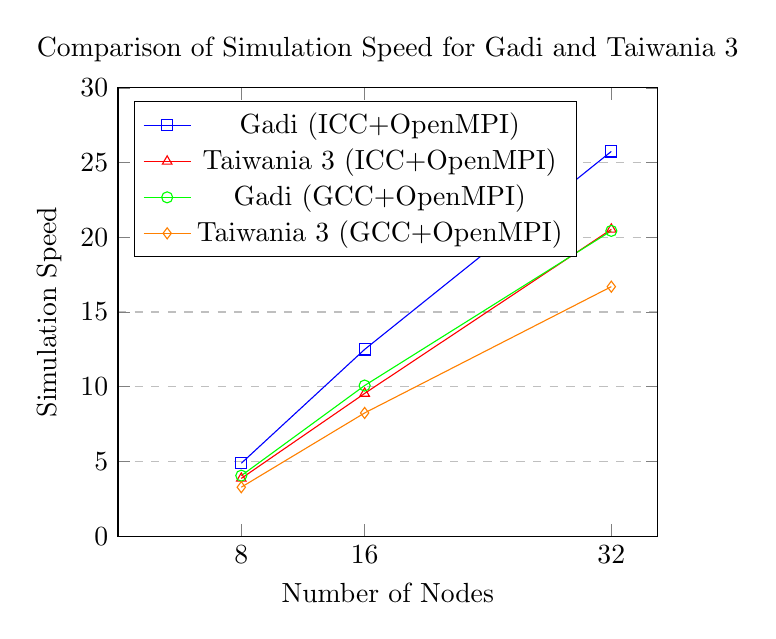
\begin{tikzpicture}
\begin{axis}[
    title={Comparison of Simulation Speed for Gadi and Taiwania 3},
    xlabel={Number of Nodes},
    ylabel={Simulation Speed},
    xmin=0, xmax=35,
    ymin=0, ymax=30,
    xtick={8, 16, 32},
    ytick={0, 5, 10, 15, 20, 25, 30},
    legend pos=north west,
    ymajorgrids=true,
    grid style=dashed,
]

% ICC + OpenMPI
\addplot[
    color=blue,
    mark=square,
    ]
    coordinates {
    (8, 4.8811)(16, 12.4976)(32, 25.7474)
    };
    \addlegendentry{Gadi (ICC+OpenMPI)}

\addplot[
    color=red,
    mark=triangle,
    ]
    coordinates {
    (8, 3.8668)(16, 9.5514)(32, 20.5316)
    };
    \addlegendentry{Taiwania 3 (ICC+OpenMPI)}

% GCC + OpenMPI
\addplot[
    color=green,
    mark=o,
    ]
    coordinates {
    (8, 4.0511)(16, 10.081)(32, 20.43)
    };
    \addlegendentry{Gadi (GCC+OpenMPI)}

\addplot[
    color=orange,
    mark=diamond,
    ]
    coordinates {
    (8, 3.2786)(16, 8.2471)(32, 16.6974)
    };
    \addlegendentry{Taiwania 3 (GCC+OpenMPI)}

\end{axis}
\end{tikzpicture}
\caption{Comparison of simulation speed between Gadi and Taiwania 3 with ICC and GCC compilers and OpenMPI on testcases with different nodes.}
\label{figure:final-result}
\end{figure}
